\pagestyle{headings}
%\mainmatter

\title{Appendices for A Generic Graph-based Neural Architecture Encoding Scheme for Predictor-based NAS}
\author{}
\institute{}
\titlerunning{Appendix}
\authorrunning{X. Ning et al.}


\maketitle

\section{Implementation of GATES}
\begin{table*}[tb]
\caption{Notations used in the batched computation of the GATES encoder.}
\label{tab:notation}
\small
\begin{center}
\begin{tabular}{cp{8cm}}
\toprule
\multirow{2}{*}{$V$} & maximum number of nodes: 7, 4, 6 for NAS-Bench-101~\cite{ying2019bench}, NAS-Bench-201~\cite{Dong2020NAS-Bench-201} and ENAS~\cite{pham2018efficient}, respectively \\
\specialrule{0em}{1pt}{4pt}
\multirow{2}{*}{$n_i$} & number of input nodes: 1, 1, 2 for NAS-Bench-101, NAS-Bench-201 and ENAS, respectively \\
\specialrule{0em}{1pt}{4pt}
$N_o$ &  number of operation primitives\\\cmidrule(lr){1-2}
$h_o$ & embedding size of operation\\
$h_i^{(k)}$ & embedding size of information in the $k$-th layer\\
$E \in \mathbb{R}^{n_i\times h^{(0)}_i}$  & the embedding of the information at the input nodes\\
$\mbox{EMB} \in \mathbb{R}^{N_o \times h_o}$ & the operation embeddings \\
\multirow{2}{*}{$W^{(k)}_o\in \mathbb{R}^{h_o \times h_i^{(k)}}$} & the transformation matrix on the operation embedding (the $k$-th layer)\\
\multirow{2}{*}{$W^{(k)}_x \in \mathbb{R}^{h_i^{(k-1)} \times h_i^{(k)}}$} & the transformation matrix on previous layer's output information (the $k$-th layer)\\\cmidrule(lr){1-2}
$b$ & batch size\\
$A \in \mathbb{R}^{b\times V\times V}$ & adjacency matrix\\
$X^{(k)} \in \mathbb{R}^{b \times V \times h_i^{(k)}}$ & the output virtual information of the $k$-th layer\\\hline
\specialrule{0em}{3pt}{3pt}
\multirow{2}{*}{$\mbox{EMB}(o) \in \mathbb{R}^{b \times V \times h_o}$} & (NAS-Bench-101) the embeddings of the operations on nodes\\
\multirow{2}{*}{$\mbox{EMB}(o) \in \mathbb{R}^{b \times V \times V \times h_o}$} & (NAS-Bench-201) the embeddings of the operations on edges\\
$n_d$& (ENAS) maximum input degree of nodes\\
\multirow{2}{*}{$\mbox{EMB}(o_d) \in \mathbb{R}^{b \times V \times V \times h_o}$} & (ENAS) the embeddings of operations on the $d$-th input edge for nodes 
\\\bottomrule
\end{tabular}
\end{center}
\end{table*}

In practice, to calculate the information propagation following the topological order of different graphs in a batched manner, we use a stack of GATES layers. In the forward process of each GATES layer, one step of information propagation is taken place at every node. The detailed formulas and implementations of one GATES layer for ``operation on node'' and ``operation on edge'' search spaces are shown as follows, and the notations are summarized in Table.~\ref{tab:notation}.

\subsubsection{Operation On Node (OON) Search Space}

For the OON case, we take the NAS-Bench-101 search space as an example. In the cell architecture, there is $n_i=1$ input node, and at most $V=7$ nodes. For batch computation, we pad zero columns and rows into the adjacent matrix to ensure that all adjacent matrices are of size $7\times7$, and also add none operations into the corresponding positions in the operation list. The calculation of the $k$-th GATES layer could be written as
\begin{equation}
\begin{aligned}
X^{(0)} &= \mbox{CONCAT}(\tilde{E}, {\bf 0}_{b \times V-n_i \times h_i^{(0)}}, \mbox{dim=1})\\
X^{(k)} &= \sigma(\mbox{EMB}(o) W^{(k)}_o) \odot (A X^{(k-1)} W^{(k)}_x)
\end{aligned}
\label{eq:gates_nasbench}
\end{equation}
where $\tilde{E} = \mbox{repeat}(E, [b, 1, 1]) \in \mathbb{R}^{b \times n_i \times h^{(0)}_i}$, and $E, \mbox{EMB}, W^{(k)}_o, W^{(k)}_x$ are trainable parameters.



In practice, we found that for the OON search space, adding a self-loop of the information propagation would lead to slightly better performance. 
\begin{equation}
    \begin{aligned}
        X^{(k)} &= \sigma(\mbox{EMB}(o) W^{(k)}_o) \odot (\tilde{A} X^{(k-1)} W^{(k)}_x) \\
        \tilde{A} &= A + I
    \end{aligned}
\end{equation}


\subsubsection{Operation On Edge (OOE) Search Space}

For the OOE search spaces, the calculation of a GATES layer could be written as
\begin{equation}
\begin{aligned}
X^{(0)} &= \mbox{CONCAT}(\tilde{E}, {\bf 0}_{b \times V-n_i \times h_i^{(0)}}, \mbox{dim=1})\\
S &= \expand(X^{(k-1)} W^{(k)}_x, 1)\\
X^{(k)} &= \mbox{SUM}(\sum_{d=1}^{n_d} \expand(A, 3) \odot \sigma(\mbox{EMB}(o_d) W^{(k)}_o) \odot S, \mbox{dim=2})
\end{aligned}
\label{eq:gates_enas}
\end{equation}
where $\tilde{E} = \mbox{repeat}(E, [b, 1, 1]) \in \mathbb{R}^{b \times n_i \times h^{(0)}_i}$, and $\expand(A, \mbox{dim})$ denotes the operation to insert a new dimension as dimension \textit{$\mbox{dim}$}.

For the search spaces where there is at most one edge between each pair of nodes (e.g., NAS-Bench-201), the above calculation could be simplified to
\begin{equation}
\begin{aligned}
X^{(0)} &= \mbox{CONCAT}(\tilde{E}, {\bf 0}_{b \times V-n_i \times h_i^{(0)}}, \mbox{dim=1})\\
S &= \expand(X^{(k-1)} W^{(k)}_x, 1)\\
X^{(k)} &= \mbox{SUM}(\expand(A, 3) \odot \sigma(\mbox{EMB}(o) W^{(k)}_o) \odot S, \mbox{dim=2})
\end{aligned}
\label{eq:gates_enas}
\end{equation}



\section{Discussion on Isomorhism}

\subsubsection{GATES maps ismorphic architectures to the same representation}
The encoding process of GATES mimics the actual computation flow: GATES uses multiplicative transforms to mimic the forward process of operations (e.g., \texttt{Conv3x3}), and uses commutative aggregation to mimic actual commutative aggregation of the feature maps.
Naturally, GATES would encode two architectures that give out the same feature map results into the same representation. That is to say, the embedding space of GATES is more meaningful. However, GATES might fail to map non-isomorphic architectures to different representations. And we leave it to future work to ameliorate this problem to further increase the discriminative power of GATES.

In the search spaces which we have experimented with (i.e., NAS-Bench-101, NAS-Bench-201, and ENAS), the combination of feature maps at internal nodes is done via addition operation, which is commutative. Therefore, for encoding the architecture, GATES also uses commutative addition to combine the ``virtual information''.
Note that if the feature map aggregation at some internal node is not commutative (e.g., concatenation), we should use a non-commutative aggregation of the virtual information too.

Another thing to note is that, in the NAS-Bench-101 and ENAS search spaces, the tensors going to the final output node in the cell are concatenated instead of being added together.
Since the concatenation operation is not commutative, different concatenation orders result in different architectures. Nevertheless, in these two search spaces, these models are equivalent through the rearrangement of channels in the following operations.
Therefore, we use addition to aggregate the information at the output node, too. We emphasize that this is a search space specific discussion.


\begin{table}[tb]
\begin{center}
\caption{The Kendall's Tau $\tau$ on 1) NAS-Bench-101 test set 2) the 7-vertex subset of the test set 3) all the isomorphic counterparts of the 7-vertex subset (without de-duplication). The last column shows the sum of the variances of the predicted scores in every isomorphic architectures group, and there are negligible numerical errors in the variance results of GATES and GCN. All the predictors are trained using the hinge pairwise ranking loss on 0.1\% of the training data.}
\label{table:iso-nb101}
\begin{tabular}{c@{\hskip 0.02\linewidth}cccc}
\toprule
\multirow{3}{*}{Encoders} & test set & 7-vertex test set & \multicolumn{2}{c}{7-vertex test set w.o. de-dup.} \\ 
& (42362) & (36064) & \multicolumn{2}{c}{(116102)} \\\cmidrule(lr){2-2}\cmidrule(lr){3-3}\cmidrule(lr){4-5}
& $\tau$   &$\tau$ & $\tau$  & Total Var.  \\\midrule
MLP~\cite{wang2018alphax}  & 0.5272 & 0.5143 & 0.4729 & 43.58    \\
LSTM~\cite{wang2018alphax} & 0.5993 & 0.5877 & 0.5656 & 18.80    \\
GCN~\cite{shi2019multi}    & 0.5790 & 0.5876 & 0.6169 & 1.16E-11 \\\hline
GATES                      & 0.7789 & 0.7724 & 0.7758 & 9.24E-12 \\ \bottomrule
\end{tabular}
\end{center}
\end{table}

We conduct a simple experiment to verify GATES's ability to map isomorphic architectures to the same representation on NAS-Bench-101.
After splitting the train and test sets, there are 36064, 6037, 256, 5 testing architectures with 7, 6, 5, 4 vertices, and 323018, 55973, 2185, 79, 6, 1 training architectures with 7 6, 5, 4, 3, 2 vertices respectively.
Since all isomorphic cell architectures are already removed in NAS-Bench-101, we generate the isomorphic architectures for the 36064 unique testing architectures with 7 vertices, and get 116102 architectures. Among the 36064 architectures, there are 20994 architectures that have isomorphic counterparts. We test different predictors trained with 0.1\% training samples on these 116k architectures and show the results in Table.~\ref{table:iso-nb101}. Since the sequence-based encoding schemes cannot map isomorphic architectures to the same representation, the ranking correlation decreases if no de-duplication procedure is carried out. The last column shows the sum of the variances of the predicted scores in every isomorphic architecture group. We can see that GATES and GCN can map isomorphic architectures to the same representation (a variance of 0 with negligible numeric errors), since only isomorphism-invariant aggregation operations are used in the encoding process.


\begin{figure}[tb]
\begin{center}
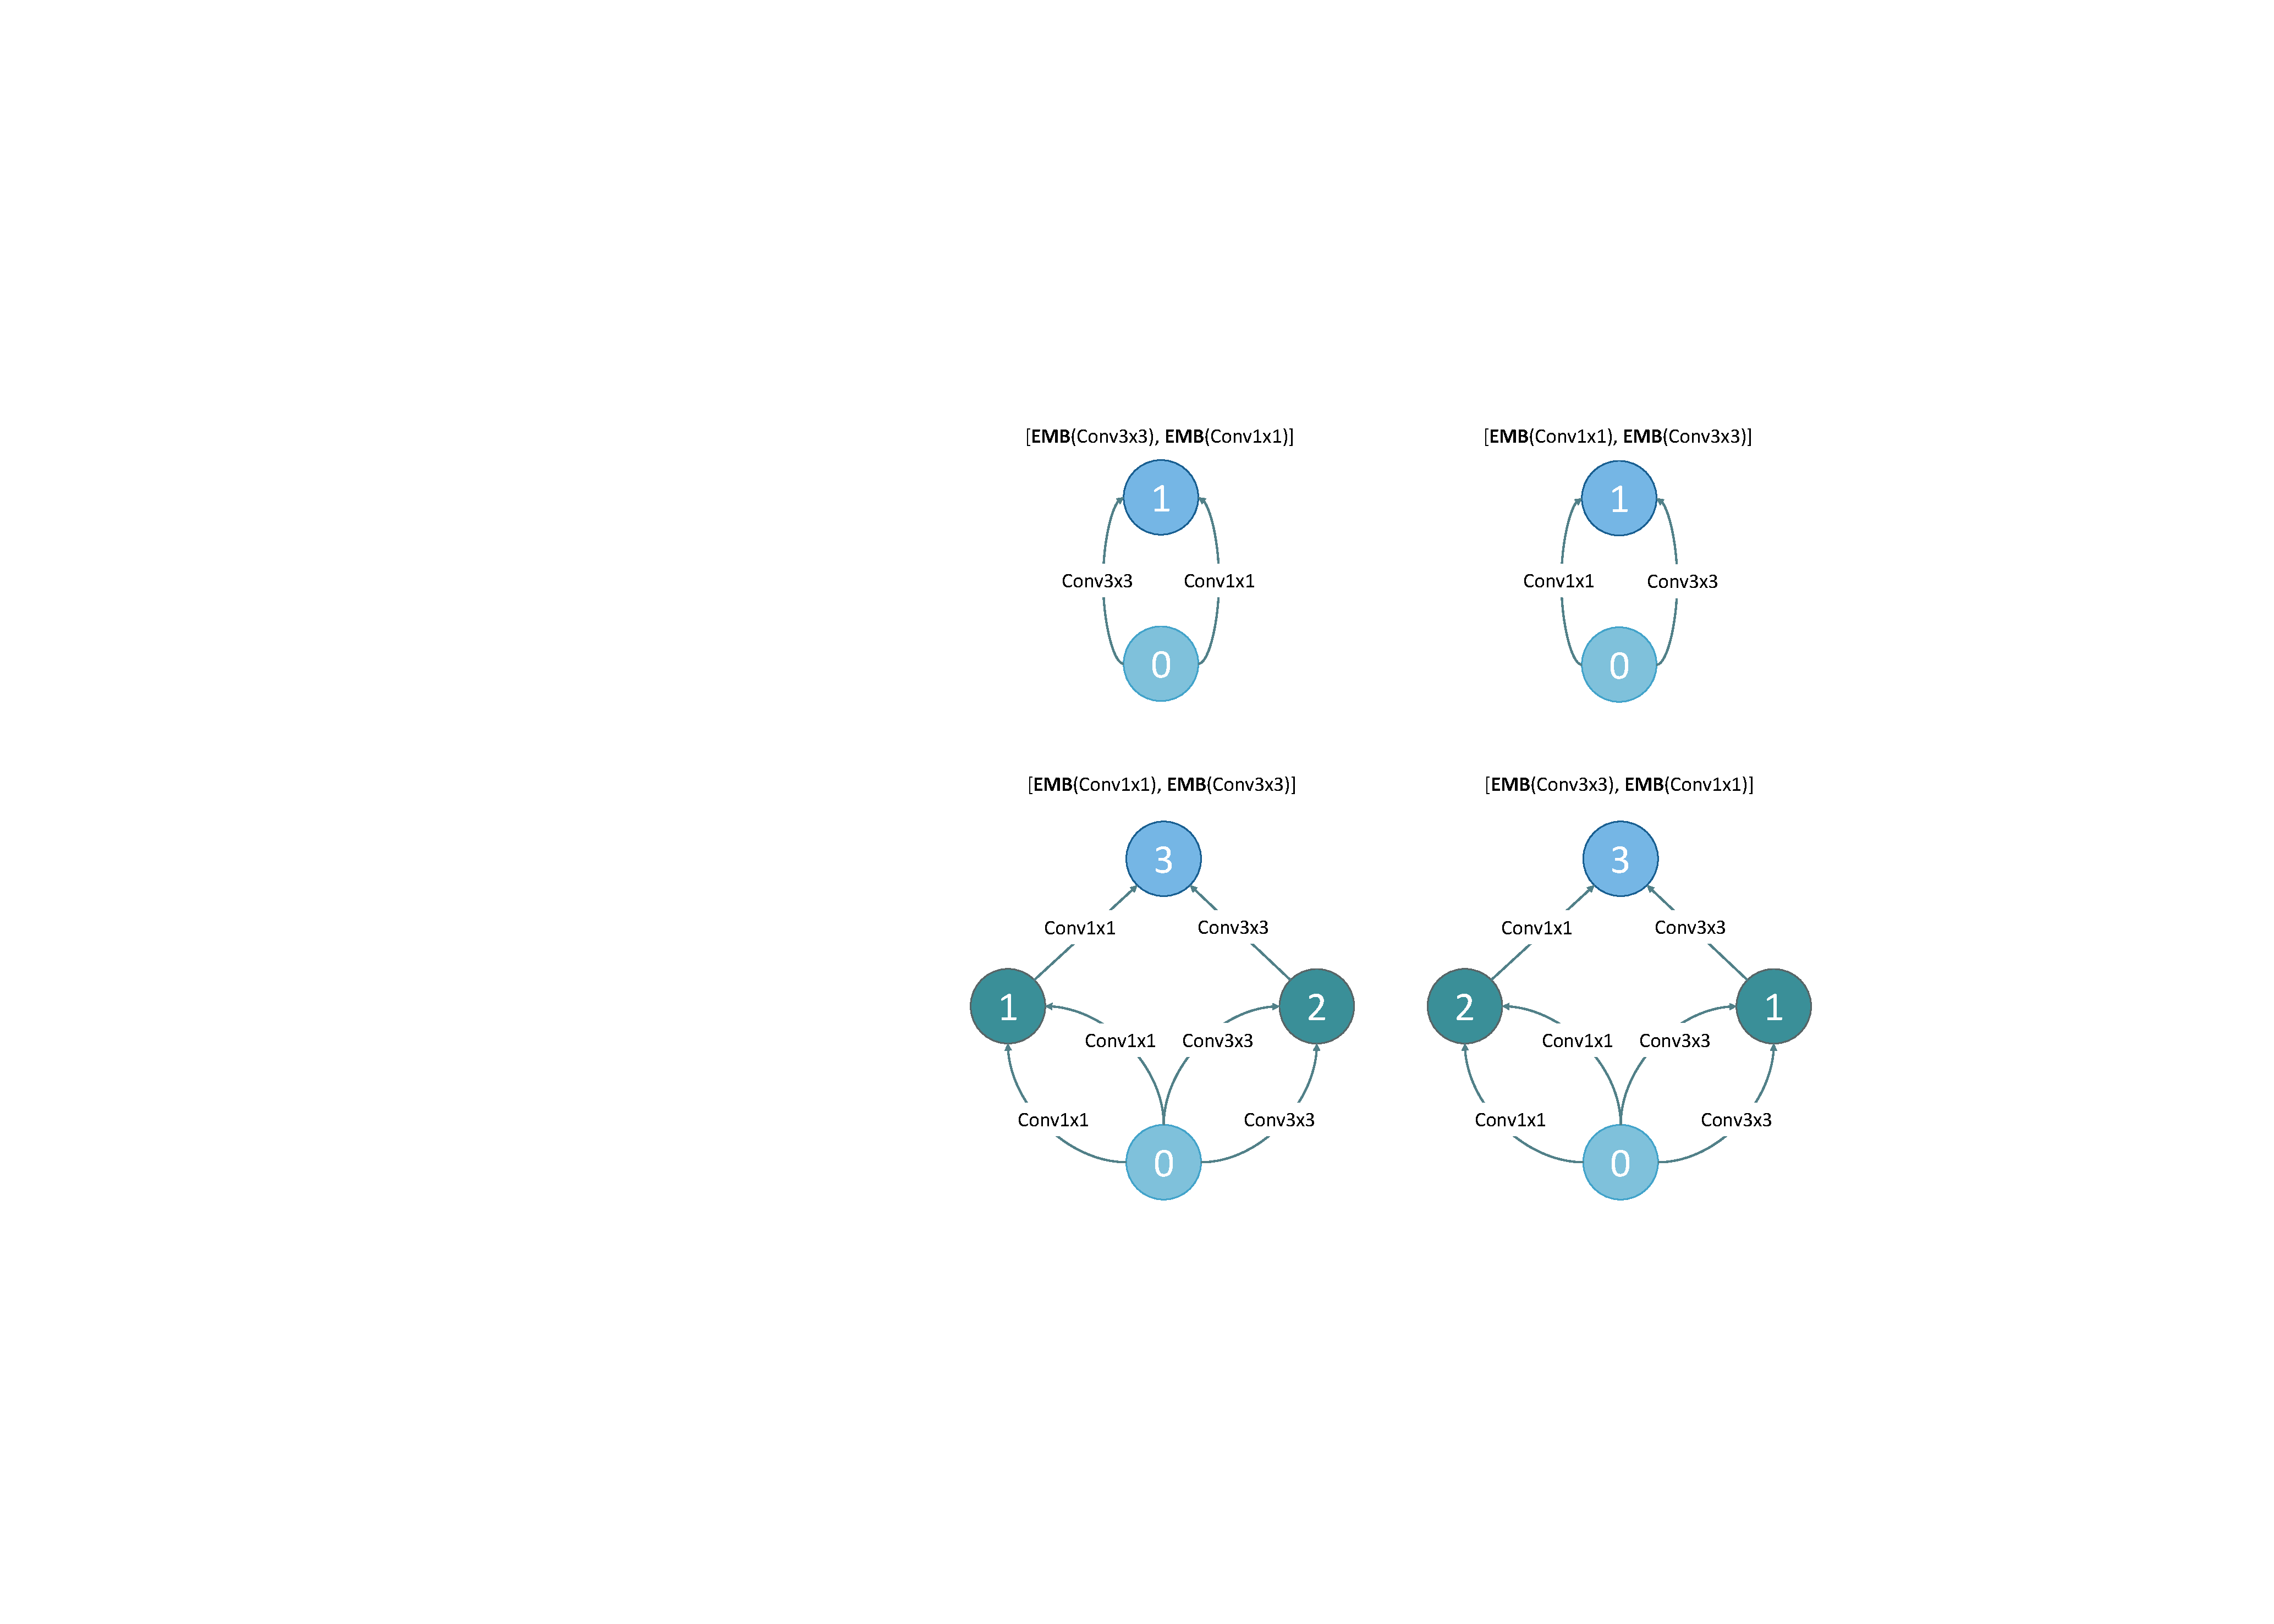
\includegraphics[width=0.64\linewidth]{figs/counter_new.pdf}
\caption{An ad-hoc graph-based solution~\cite{guo2019nat} for encoding the architecture in the ENAS search space (an OOE search space) fails to map isomorphic architectures to the same representation. In the upper case, the two architectures are the same graph, but the embeddings of Node 1 differ. This case could be solved by imposing an order of the operations when the two incoming edges come from the same previous node. In the lower case, these two architecture are isomorphic, since the feature map aggregation at Node 3 is a commutative element-wise addition. However, this encoding scheme cannot guarantee to map these two architectures to the same representation, since the original node embeddings already differ at Node 3. The failure to handle the isomorphism is due to the non-commutative characteristics of the concatenation operation.}
\label{fig:guo_gcn_counter_example}
\end{center}
\end{figure}

\subsubsection{Two counter examples of the ad-hoc solution~\cite{guo2019nat}}
Since GCN cannot be directly applied to encoding architectures from the OOE search spaces, a recent study~\cite{guo2019nat} proposes an ad-hoc solution for the ENAS search space. They represent each node by the concatenation of the operation embeddings on the input edges. This solution cannot generalize to search spaces where nodes could have different input degrees. What’s more, since the concatenation operation is not commutative, this encoding scheme could not map isomorphic architectures to the same representation correctly. Fig.~\ref{fig:guo_gcn_counter_example} illustrates two minimal counterexamples.

\section{Setup and Additional Results}

\subsubsection{Setup and Results on NAS-Bench-101}
The setup of all the experiments on NAS-Bench-101 goes as follows. An ADAM optimizer~\cite{kingma2014adam} with learning rate 1e-3 is used to optimize the performance predictors for 200 epochs. And the average of the ranking correlations in the last 5 epochs is reported. The batch size is set to 512. And a hinge pairwise ranking loss with margin 0.1 is used. For the construction of the MLP and LSTM encoder, we follow the serialization method and the model settings in \cite{wang2018alphax}. The MLP is constructed by 4 fully-connected layers with 512, 2048, 2048, and 512 nodes, and the output of dimension 512 is used as the cell's embedding. The embedding and hidden sizes of the LSTM are both set to 100, and the final hidden state is used as the cell's embedding. For the GCN and GATES encoders, we construct the encoder by stacking five 128-dim GCN or GATES layers. 
All the embedding sizes are set to 48, including the operation embedding in GCN, and the operation and information embedding in GATES. For GCN, the average of all the nodes' features is used as the cell's embedding. In GCN with global node~\cite{shi2019multi}, the features of the global node are used as the cell's embedding.

Fig.~\ref{fig:scatter-nb101} shows the prediction results on the 42362 testing architectures with different encoders trained on 0.1\% training data.
As can be seen, compared with the GCN and MLP encoders, the predictions of GATES are much more accurate in the sense of ranking correlation.


\begin{figure*}[bt]
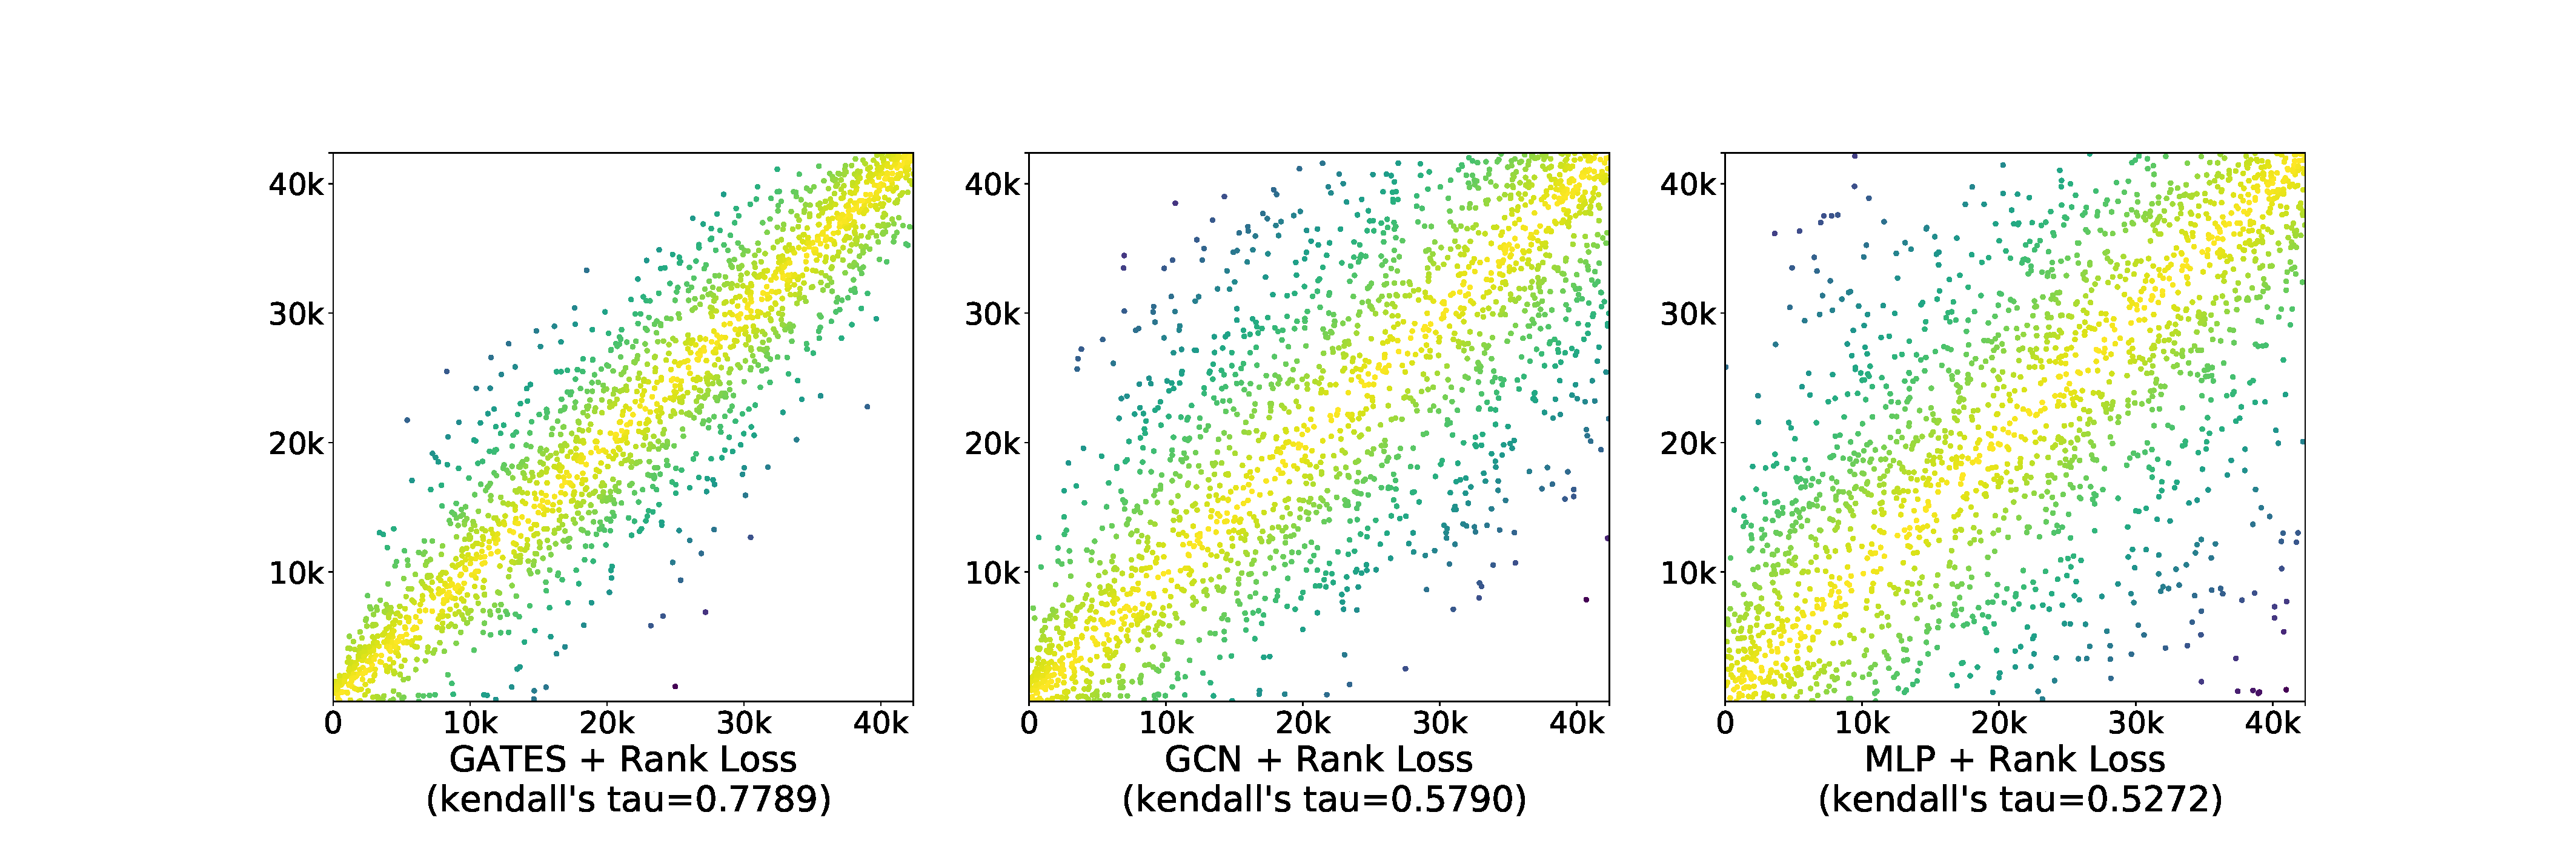
\includegraphics[width=1.\linewidth]{figs/nb101_sactter.pdf}
\caption{NAS-Bench-101: The true rankings (y-axis) and predicted rankings (x-axis) of 2000 architectures among the 42362 testing architectures. 0.1\% training data are used to train these encoders.}
\label{fig:scatter-nb101}
\end{figure*}

\subsubsection{Setup on NAS-Bench-201}
The setup of all the experiments on NAS-Bench-201 goes as follows. An ADAM optimizer with learning rate 1e-3 and batch size 512 is used to train the predictors for 200 epochs, and the average of testing Kendall's Taus in the final 5 epochs is reported.

For the sequence-based baselines (MLP and LSTM), we use the 6 elements of the lower triangular portion, excluding the diagonal ones. We use 4 fully-connected layers with 512, 2048, 2048, 512 nodes for the MLP encoder. The embedding size and hidden size of the 1-layer LSTM is set to 100, and the final hidden stage is used as the embedding of the cell architecture. As for GATES, we use a 5-layer GATES encoder without self-loop.


\subsubsection{Neural Architecture Search in the ENAS Search Space}


The setup of the predictor training goes as follows. The predictor is constructed by four 64-dim GATES layers. Both the operation and information embedding sizes are set to 32. During the training of the predictor, the total epoch is set to 80, and the batch size is set to 128, and a pairwise hinge loss with margin 0.1 and an ADAM optimizer with learning rate 1e-3 are used.

For the true performance evaluation of the 800 architectures (600 randomly sampled, 200 sampled utilizing the predictor), we train them for 80 epochs using an SGD optimizer with weight decay 3e-4. The learning rate is decayed from 0.05 to 0.001 following a cosine schedule. The base channel number is 16, and the number of layers is 8.

The discovered architecture is shown in Fig.~\ref{fig:enas_discover_cell}. To evaluate the final performance of the discovered cell architecture, we first apply the channel and layer augmentation. Specifically, 20 cells are stacked to construct the network, and the base channel number is increased from 16 to 36. The augmented model is trained for 600 epochs on CIFAR-10 with batch size 128, and the learning rate is decayed from 0.05 to 0.001 following a cosine schedule. The cutout data augmentation with length 16 is used. The weight decay is set to 3e-4, and the dropout rate before the fully-connected classifier is set to 0.1. For other regularization techniques, we follow existing studies~\cite{zoph2018learning,darts} to use auxiliary towers with weight 0.4 and the scheduled drop-path of probability 0.2. 



\begin{figure}[th]
  \begin{center}
    \subfigure[Normal cell]{
      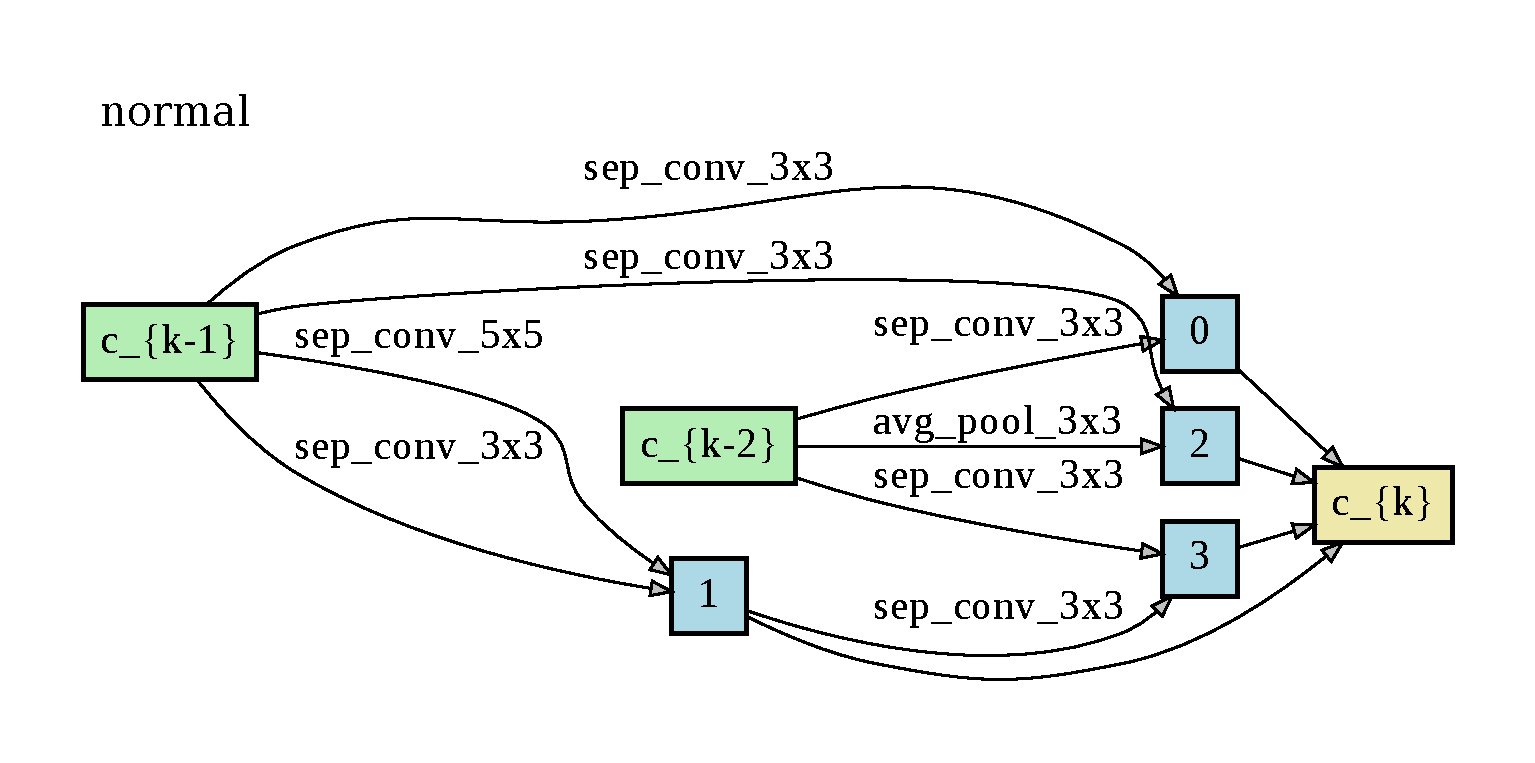
\includegraphics[width=0.75\linewidth]{figs/cell_normal.pdf} 
    }
    \subfigure[Reduction cell]{
      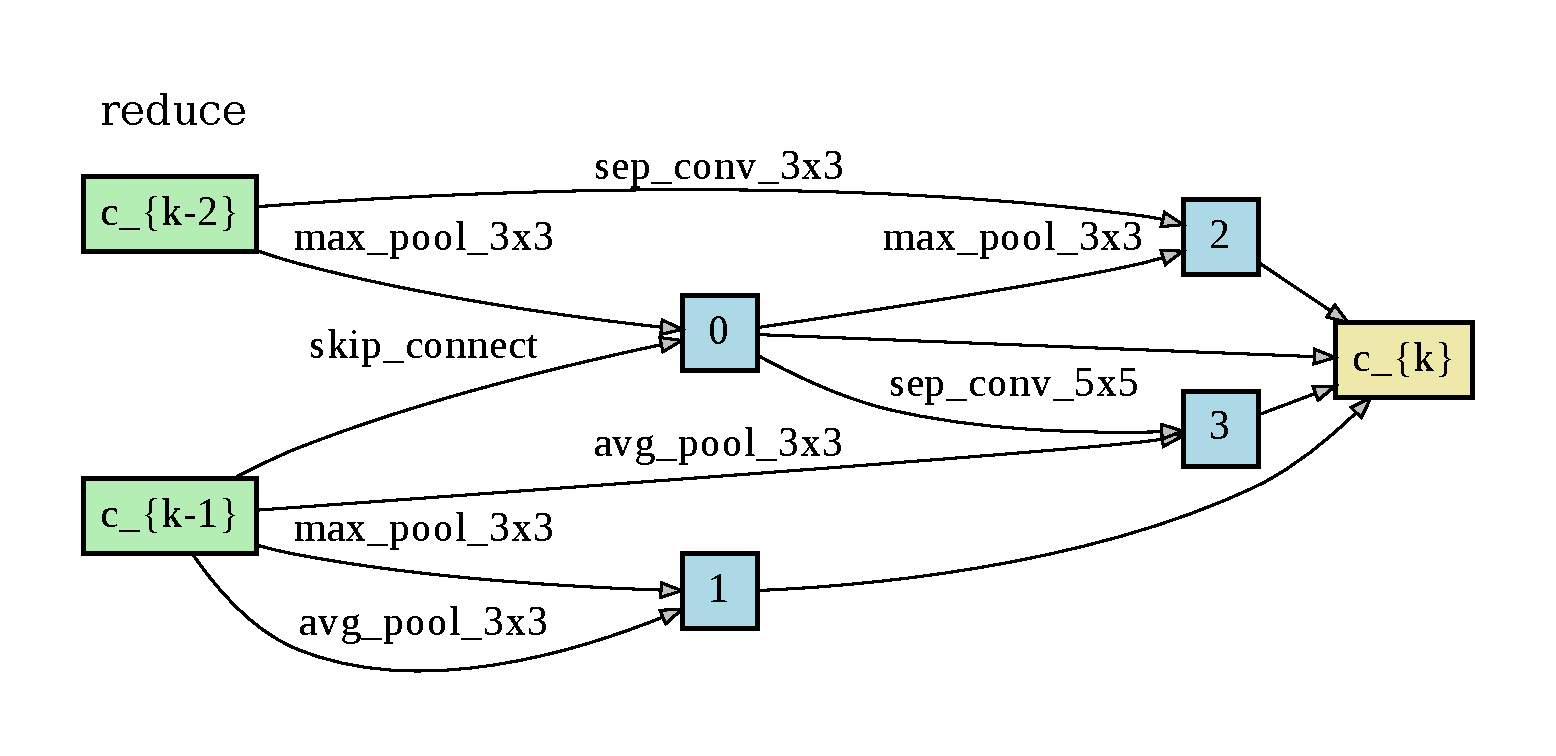
\includegraphics[width=0.75\linewidth]{figs/cell_reduce.pdf} 
    }
    \caption{Discovered cell architectures on CIFAR-10.}
    \label{fig:enas_discover_cell}
  \end{center}
  \vspace{-5pt}
\end{figure}

\section{Ranking Losses for Predictor Optimization}

The ranking correlation of the performance predictor on unseen architectures is the key to the success of predictor-based NAS. 
Since ranking losses are better surrogates of the ranking measures than the regression loss~\cite{chen2009}, training the performance predictor with ranking losses could lead to better ranking correlation.

We utilize different pairwise and listwise ranking losses for training the predictor~\cite{burges2005learning,shashua2003ranking,xia2008listwise}. The pairwise ranking loss could be written as
\begin{equation}
    \begin{aligned}
    L^p(\tilde{S})= \sum_{i=1}^{N} \sum_{j \in \{j | y_i < y_j\}} \phi(P(a_j), P(a_i))
    \end{aligned}
\end{equation}


We experiment with two different choices of $\phi$. 1) The binary cross entropy function $\phi(s_j, s_i)=\log(1 + e^{(s_j - s_i)})$; 
2) The hinge loss function $\phi(s_j, s_i)= \max(0, m - (s_j - s_i))$, where $m$ is a positive margin.

We also experiment with a pairwise comparator: We construct an MLP that takes the concatenation of two architecture embeddings as input and outputs a score: $s=\mbox{MLP}([E(a_j), E(a_i)]$, and a positive $s$ indicates that $a_j$ is better than $a_i$.  Note that the total-orderness of the architectures is not guaranteed using this comparator. So, we add a simple anti-symmetry regularization term in the training of the comparator. The loss for training the comparator is:
\begin{equation}
    \begin{aligned}
    L^p(\tilde{S})= &\sum_{i=1}^{N} \sum_{j \in \{j | y_i < y_j\}} \max(0, m - \mbox{MLP}([E(a_j), E(a_i)]) \\
    &+ \max(0, m + \mbox{MLP}([E(a_i), E(a_j)]))
    \end{aligned}
\end{equation}


We design the listwise ranking loss following ListMLE~\cite{xia2008listwise}:
\begin{equation}
    L^l(\tilde{S}) = \sum_{U \subset \tilde{S}} \sum_{i=1}^{|U|} \{-P(a^{(i), U}) + \log\sum_{j=i}^{|U|} \exp(P(a^{(j), U}))\}
\end{equation}
where $U$ are subsets of $\tilde{S}$, $|U|$ denotes the size of $U$, $a^{(i), U}$ denotes the architecture whose true performance $y^{(i), U}$ is the $i$-th best in the subset $U$.

\subsection{Evaluation of Ranking Losses}
\subsubsection{Setup}


In the experiments of evaluating the ranking losses, the training settings and the construction of the GATES model are the same as in the evaluation of GATES. 
One exception is that, for the listwise ranking loss (ListMLE), we train the predictor for 80 epochs (list length is 4), since the training converges much faster with the listwise ranking loss. Still, the average of the ranking correlations in the last 5 epochs is reported.

The evaluation of the comparator-based ranking loss is a little different than other ranking losses. For other ranking losses, we can calculate the ranking correlation between the predicted scores $\mbox{P}(a)$ and the true accuracies. However, a comparator trained using the comparator-based ranking loss must take a pair of architectures as the input and output a comparison results. Therefore, for evaluating the performance of the comparator,
we run the randomized quick-sort procedure with the comparator to get the predicted rankings of the testing architectures. Since the comparator might not be a proper total order operator, different choices of the random pivots in randomized quick-sort could lead to different sorted sequences. Therefore, we run randomized quick-sort with 3 different random seeds, and report the average Kendall's Tau. In practice, we find that the Kendall's Taus calculated using different random seeds are very close. For example, three tests with random seed 1, 12 and 123 of the predictor trained on the whole training set give the Kendall's Taus of 0.90106, 0.90107 and 0.90113, respectively.



\begin{table*}[tb]
  \vspace{-5pt}
  \caption{The Kendall’s Tau of using different loss functions on NAS-Bench-101. The first 90\% (381262) architectures in the dataset are used as the training data, and the other 42362 architectures are used as the testing data. All experiments except ``Regression (MSE) + GCN'' are carried out with GATES encoder.}
  \label{table:rank-nb101}
  \begin{center}
    \resizebox{0.96\textwidth}{!}{
      \begin{tabular}{ccccccccc}
        \toprule
        \multirow{2}{*}{Loss} & \multicolumn{8}{c}{Proportions of 381262 training samples}\\ 
        \cmidrule(lr){2-9} & 0.05\% & 0.1\% & 0.5\% & 1\% & 5\% & 10\% & 50\%  & 100\% \\ \midrule
        Regression (MSE) + GCN$^\dagger$ &0.4536 & 0.5058 & 0.5587 & 0.5699 & 0.5846 & 0.5871 & 0.5901 & 0.5941\\
        Regression (MSE) + GATES$^\dagger$ & 0.4935 & 0.5425 & 0.5739 & 0.6323 & 0.7439 &  0.7849 &  0.8247 & 0.8352\\\hline
        Pairwise (BCE) & 0.7460 & 0.7696 & 0.8352 & 0.8550 & 0.8828 & 0.8913 &  0.9006 & 0.9042 \\
        Pairwise (Comparator) & 0.7250 & 0.7622 &  0.8367 & 0.8540 & 0.8793 & 0.8891 &  0.8987 & 0.9011\\
        % eva10:~/projects/aw_nas_clones/aw_nas_comparator/scripts/nasbench/results_nasbench101/full/pairwise_gatesplusI/gatesx5plusI_nt_comparator/tr1.0e+00/train.log
        Pairwise (Hinge) & 0.7634 & 0.7789 & 0.8434 & 0.8594 & 0.8841 & 0.8922 &  0.9001& 0.9030 \\
        Listwise (ListMLE) & 0.7359 & 0.7604 & 0.8312 & 0.8558 & 0.8852 & 0.8897 &  0.9003 & 0.9009\\\bottomrule
        % /home/eva_share/foxfi/aw_nas_new/scripts/nasbench/results_nasbench101/listwise/train_ratio_ts10_ll
      \end{tabular}
    }
    \begin{minipage}{1.0\textwidth}
      {\small
        $\dagger$: For the baseline evaluation of regression loss, we use a GCN encoder with 1 layer, and a GATES encoder with 3 layers rather than 5 layers, since training deep GCN or GATES encoder with MSE regression loss is unstable, and often fails to learn anything meaningful. With MSE loss, 1 layer of GCN and 3 layers of GATES achieve the best results among layer number configurations using 0.1\% training data.
      }
    \end{minipage}
  \end{center}
  \vspace{-10pt}
\end{table*}

\subsubsection{Results on NAS-Bench-101}
We train GATES-powered predictors with four types of ranking losses: 1) Pairwise loss with binary cross-entropy $\phi$. 2) Pairwise loss with a hinge loss function $\phi$. 3) Pairwise comparator loss. 4) Listwise (ListMLE).
Table~\ref{table:rank-nb101} shows the comparison of using different losses to train the predictors on NAS-Bench-101. Compared with the regression loss, ranking losses bring consistent improvements.
The performances of different ranking losses are close, and the pairwise hinge loss is a good choice. We also find that training with regression loss requires a smaller learning rate and longer time to converge, and does not work well with 
deep GCN or GATES models.

\subsubsection{Results on NAS-Bench-201}
Table~\ref{table:gates-nb201} shows the comparison of using regression and ranking losses to train the predictors on NAS-Bench-201. We can see that training using ranking losses leads to better-correlated predictors consistently.

\addtolength{\tabcolsep}{1pt}
\begin{table*}[tb]
  \vspace{-5pt}
\caption{The Kendall’s Tau of using different encoders and loss functions on NAS-Bench-201. The first 50\% (7813) architectures in the dataset are used as the training data, and the other 7812 architectures are used as the testing data}
\label{table:gates-nb201}
\begin{center}

\begin{tabular}{cccccc}
\toprule
\multirow{2}{*}{Encoder} & \multicolumn{5}{c}{Proportions of 7813 training samples}\\ 
\cmidrule(lr){2-6} & 1\% & 5\% & 10\% & 50\% & 100\% \\\midrule
MLP + Regression (MSE)$^\dagger$ & 0.0646 & 0.1520 & 0.2316 & 0.5156 & 0.6089  \\
LSTM + Regression (MSE) & 0.4405 & 0.5435 & 0.6002 & 0.8169 & 0.8614\\
GATES + Regression (MSE) & 0.6823 & 0.7528 & 0.8042 & 0.8950 & 0.9115\\\hline
MLP + Pairwise (Hinge)  &  0.0974 & 0.3959 & 0.5388 & 0.8229 & 0.8703\\
LSTM + Pairwise (Hinge) & 0.5550 & 0.6407 & 0.7268 & 0.8791 & 0.9002\\
  GATES + Pairwise (Hinge) & 0.7401 & 0.8628 & 0.8802 & 0.9192 & 0.9259\\\bottomrule

\end{tabular}
\begin{minipage}{1.0\textwidth}
{\small
$\dagger$: For the baseline evaluation of MSE regression loss + MLP encoder, we use a learning rate of 1e-4, since we find out that MLP cannot be learned with 1e-3 learning rate.% of 1e-3.
}
\end{minipage}
\end{center}
\vspace{-5pt}
\end{table*}
\addtolength{\tabcolsep}{-1pt}

